\section{Резонанс на виртуальном электроне}\label{sec:resonance}
\subsection{Резонанс в комптоновском рассеянии}
Интерес к изучению комптоновского рассеяния $\gamma e \to \gamma e$ в 
сильном магнитном поле первоначально был вызван неожиданным открытием циклотронных 
спектральных линий у двойных рентгеновских 
пульсаров~\cite{Truemper1978,Makishima1990,Grove1995}, которые изначально 
интерпретировались либо как циклотронное поглощение, либо как циклотронное 
излучение~\cite{Truemper1978}. Дальнейшее повышение разрешения детекторов по 
энергии позволило уверенно заключить, что циклотронные особенности связаны 
именно с резонансным поглощением фотона~\cite{Mihara:1990}.
При этом под циклотронным резонансом обычно понимается 
резкое увеличение сечения рассеяния по сравнению с классическим томсоновским 
сечением $\sigma_T = 8 \pi \alpha^2 /(3 m^2)$. В одной из первых 
работ по этой тематике~\cite{Canuto:1971} выражение для сечения 
комптоновского 
рассеяния в магнитном поле без плазмы было получено
в нерелятивистском пределе, и для фотона, 
распространяющегося вдоль магнитного поля, в сечении был обнаружен резонансный 
пик при энергии:
\begin{equation}\label{eq:w_B}
	\omega_B\simeq \frac{\beta}{m}.
\end{equation}
 
Кроме того, в работе~\cite{Canuto:1971} также было показано, что сечение рассеяния фотона 
на электроне
значительно зависит как от поляризационного состояния фотона, так и от угла 
между направлением импульса начального фотона и направлением магнитного поля. В 
последовавшей за ней 
статье~\cite{Gnedin1973} 
исследовалось изменение энергии фотона в комптоновском процессе, кратное 
циклотронной частоте $\omega_B$. 
В следующих работах~\cite{Borner1979,Ventura:1979} 
были получены результаты для полного сечения рассеяния фотона на электроне с использованием формализма работы~\cite{Canuto:1971}. Тем не менее эти результаты будут справедливыми только для относительно слабого магнитного поля~$B<10^{12}$~Гс. Однако при значениях магнитного поля~$B>10^{12}$~Гс, как было показано в работах~\cite{Herold:1979,Melrose:1983III},   учет релятивистских эффектов в сечении комптоновского рассеяния становится 
существенным.

В представленных выше работах предполагалось, что начальный и конечные электроны находятся 
на основном уровне Ландау, что является справедливым для предела сильного магнитного поля 
и/или низких температур $T\ll m$ (см. Введение). В этом случае резонансный 
пик~(\ref{eq:w_B})  смещается в область более низких энергий фотона, а кроме 
него возникает бесконечный ряд резонансных пиков, соответствующих разным 
уровням Ландау $n$ 
виртуального электрона. Эти пики реализуются при энергиях фотона:
\begin{equation}\label{eq:whn}
	\omega_n(\theta)= \frac{\sqrt{m^2+2 \beta n \sin^2\theta} - 
		m}{\sin^2\theta}\, ,
\end{equation}
где $\theta$ -- угол между импульсом начального фотона и направлением 
магнитного поля. 

С другой стороны, в результате комптоновского процесса могут возбуждаться 
высшие уровни Ландау начального электрона, что, в свою очередь, может выступать 
механизмом рождения фотонов малых энергий для магнитных полей $B\lesssim 
B_e$~\cite{Daugherty:1986,Bussard:1986}. В таком случае для произвольных уровней Ландау $\ell$ начального электрона резонансные 
пики будут наблюдаться на энергиях:

\begin{equation}\label{eq:resAll}
	\omega_{n\ell}(\theta)=\frac{\sqrt{M_\ell^2 - \sin^2\theta (M_\ell^2-M_n^2)}-M_\ell}{\sin^2\theta}\, ,
\end{equation}
где $M_\ell=\sqrt{m^2+2\beta \ell}$, $M_n=\sqrt{m^2+2\beta n}$ и т.п.

В рассмотренных выше работах сечение комптоновского рассеяния 
становится бесконечным при энергиях фотона, соответствующих циклотронным 
резонансам~(\ref{eq:whn}) вследствие предположения о 
большом времени жизни виртуальных частиц. По этой причине их результаты 
справедливы только для областей энергий фотона вдали от резонансов
и могут быть применены, например, для моделирования излучения 
замагниченной 
	холодной плазмы вблизи поверхности нейтронных 
	звезд~\cite{Ozel:2001} или же для относительно слабых магнитных 
	полей $B\lesssim 10^{10}$ Гс~\cite{Zavlin:1996}.

С другой стороны, учет резонансов в комптоновском процессе является необходимым 
при моделировании спектров излучения сильно замагниченных нейтронных 
звезд~\cite{Alexander:1991,Araya:1999,Ho:2001,Lyutikov:2006,Potekhin:2004,Schonherr:2007,Nishimura:2008,Suleimanov:2009}.
Вблизи поверхности нейтронной звезды, где формируется излучение, резонансный 
обратный комптоновский процесс рассеяния фотонов малых энергий на высокоэнергетических электронах 
является доминирующим процессом, который приводит к охлаждению плазмы 
внутренней магнитосферы и образованию высокоэнергетического хвоста в спектре 
излучения~\cite{Fernandez:2007,Nobili:2008,Baring:2018,Beloborodov:2013}.
%Ozel2001: Перенос излучения сильно замагниченой атмосферы НС и конструирование излучательно равновесные модели для спектра. Атмосфера полностью ионизирована с идеальным газом в локальном термодинамическом равновесии. Атмосфера тонкая. 10^13<B<10^15. Предел холодной плазмы.
%Zavlin:1996 Слабые поля для разного химического состава.
%

Вблизи 
циклотронных резонансов для расчета сечения 
комптоновского рассеяния требуется учесть полную 
ширину изменения состояния электрона. В нерелятивистском 
пределе~\cite{Canuto:1971} присутствует лишь одна резонансная 
частота~(\ref{eq:whn}) и сечение рассеяния
не зависит от поляризационного состояния электрона (или его спинового состояния), 
поэтому ввести полную ширину относительно просто~\cite{Daugherty:1989}. Однако 
в сильных магнитных полях~$B\gtrsim B_e$ и при высоких энергиях частиц 
требуется учитывать релятивистские поправки, что приводит к тому, что выражение 
для  сечения 
становится очень громоздким, поскольку оно имеет бесконечное число 
резонансов~(\ref{eq:resAll}), 
содержащихся в сумме по всем промежуточным виртуальным состояниям.

Изначально для учета конечных резонансных пиков использовались усредненные по спину ширины распада промежуточного состояния~\cite{Gonthier:2000, Holodov:2000}. 
Как было указано в работе~\cite{Gonthier:2014}, такой подход не является 
точным, поскольку усреднение по спину некорректно учитывает спиновую 
зависимость времени распада виртуального электрона, что приводит к неверному значению сечения комптоновского рассеяния в точке 
резонанса. Этот недостаток был устранен в работе~\cite{Mushtukov:2016}, где 
представлено сечение рассеяния процесса $\gamma e\to \gamma e$ с учетом 
ширины распада виртуальных промежуточных состояний, которая 
зависит от 
поляризационного состояния электрона. 
Однако полное сечение комптоновского рассеяния, полученное таким методом, 
представляет собой громоздкое выражение, что, например, затрудняет его 
использование в моделях переноса излучения. 

В ряде случаев выражение сечения рассеяния можно упростить для получения 
аналитического 
решения различных задач. 
Так, в работе~\cite{Gonthier:2000} была использована 
аппроксимация сечения рассеяния с учетом резонанса в ультрарелятивистском 
пределе для случая относительно сильного магнитного поля $B>0.1 B_e$. В точке 
циклотронного резонанса виртуальный электрон становится реальным и распадается 
на масштабе комптоновского времени, поэтому вероятность
комптоновского рассеяния сводится к вероятности одновершинного процесса 
поглощения фотона электроном $\gamma 
e \to e$. В 
работе~\cite{Harding:1991} исследовался вопрос аппроксимации комптоновского 
сечения с помощью одновершинного процесса поглощения фотона электроном для 
магнитных полей 
$B\sim 
0.1B_e$. При этом различие между одновершинным процессом поглощения и комптоновским 
рассеянием становится существенным на высших циклотронных резонансах из-за 
нерезонансного вклада. Еще один подход рассмотрен в 
работе~\cite{Rumyantsev:2017}, он заключается в том, что пропагатор 
виртуального электрона можно заменить 
на дельта-функцию, когда основной вклад 
в сечение рассеяния будут давать области вблизи резонансов (приближение узкого 
пика). 
 
Далее рассмотрим получение сечения рассеяния комптоновского процесса в случае узкого резонансного пика.
Лагранжиан взаимодействия электрона с фотоном может быть представлен в виде:
%
\begin{eqnarray}\label{eq:L}
	{\cal L}(X) \, = \,- e [\bar \Psi (X) \gamma^{\mu} A^{(\lambda)}_\mu (X) 
	\Psi(X)] \, ,
	\label{eq:Lel}
\end{eqnarray}
%
\noindent где $\Psi (X)$ -- волновая функция электрона~(\ref{eq:FermionWaveF}), 
$A^{(\lambda)}_\mu (X)$ -- волновая функция  фотона 
в виде плосковолновых 
решений:
%
\begin{eqnarray}
	\label{eq:j_k}
	A^{(\lambda)}_\mu (X) = \frac{e^{-\ii(qX)}}{\sqrt{2q_0 V}} \, \varepsilon^{(\lambda)}_\mu(q) \, ,
\end{eqnarray}
\noindent  $V = L_x L_y L_z$ -- нормировочный объем и $\lambda = 1, 2$ -- мода 
фотона.

$S$-матричный элемент рассеяния фотона поляризации $\lambda$ на электроне с рождением электрона и фотона поляризации $\lambda'$, с учетом лагранжиана~(\ref{eq:L}) может быть представлен в виде:  
%
\beq                          
\nonumber
{\cal S}^{s^{\, \prime} s}_{\gamma^{(\lambda)} e \to \gamma^{(\lambda')} e'} 
&=& - e^2\int \dd^4 X \dd^4 Y A^{(\lambda)}_\mu (X) A^{(\lambda')}_{\mu'} (Y)
%\times 
%\\[3mm]
%\nonumber
%&\times& 
\, \left [\bar \Psi^{s'}_{p',\ell'}(Y) \gamma_{\mu'} 
S^{s''}_n (Y,X) 
\gamma_\mu \Psi^{s}_{p,\ell}(X) \right ]\, +
\\[3mm]
\label{eq:S1a}
&+& (A^{(\lambda)}_\mu, \gamma_\mu \leftrightarrow A^{(\lambda')}_{\mu'}, \gamma_{\mu'})\, .
\eeq

Если в области резонанса выполняется условие 
$E_n''\Gamma^{s''}_n\ll \left|(p+q)^2_{\mprl}-M_n^2\right|$, где 
$E_n''=E_n+\omega$ -- энергия виртуального электрона, то 
можно 
использовать 
приближение узкого резонансного пика. Здесь $\Gamma^{s''}_n$ -- полная ширина 
изменения состояния электрона за счет процесса рассеяния фотона на электроне, 
которую можно выразить через ширину поглощения электрона в процессе $e_n \to 
e_{\ell'} \gamma$~\cite{Weldon:1983}:
\begin{eqnarray}
	\label{Gns}
	\Gamma_n^{s''} \simeq 
	\Gamma^{(abs) \, s''}_{e_n  \to e_{\ell'}\gamma} 
	\left [1+ \eee^{-(E_n'' - \mu)/T} \right ]\, ,
\end{eqnarray}
%
\beq
\label{eq:e_abs}
\Gamma^{(abs) \, s''}_{e_n \to e_{\ell'} \gamma}  &=& \sum\limits_{\ell' = 
	0}^{n-1} \;  \sum\limits_{s' = \pm 1} \; \sum\limits_{\lambda'} \; 
\int \frac{\dd p'_y \dd p'_z  L_y L_z }{(2\pi)^2} \,[1 - f_{e}(E^{\, 
	\prime}_{\ell'})] \times 
\\
\nonumber
&\times& \frac{\dd^3 q' V}{(2\pi)^3} \, (1 + f_\gamma(\omega')) \;
\frac{|{\cal S}^{s^{\,\prime} s''}_{e_n \to e_{\ell'} 
		\gamma^{(\lambda')}}|^2}{\tau}\, ,
\eeq 
где $f_{e}(E^{\, 
	\prime}_{\ell'})=(1+\exp [E^{\, 
	\prime}_{\ell'}/T])^{-1}$ -- равновесная функция распределения электронов с 
	температурой $T$ и нулевым химическим потенциалом, 
	$f_\gamma(\omega')=(\exp 
	[\omega'/T]-1)^{-1}$ -- равновесная функция распределения фотонов.
В приближении узкого резонансного пика квадрат знаменателя
пропагатора~(\ref{eq:propagator}) может быть заменен на $\delta$-функцию:
\begin{equation}
	\label{gamma_factor}
	\left|\frac{1}{(p+q)^2_{\mprl}-M_n^2-\ii E_n''\Gamma^{s''}_n/2}\right|^2
	\simeq\frac{2\pi}{E_n''\Gamma_n^{s''}} \delta((p+q)^2_{\mprl}-M_n^2).
\end{equation}


С учетом этого квадрат $S$-матричного элемента, определяющий вероятность процесса и необходимый при расчетах вычисляемых величин, таких как сечение рассеяния, может быть представлен в факторизованном виде:
%
\beq
\label{eq:S2factor1}
\sum\limits_{s, s' = \pm 1} \frac{|{\cal S}^{s^{\,\prime} s}_{{\gamma^{(\lambda)} e_\ell \to \gamma^{(\lambda')} e_{\ell'}}}|^2}{\tau} = 
\sum\limits_{s, s', s'' = \pm 1} 
\sum\limits_{n=0}^{\infty} \;  \int \frac{\dd p^{\, \prime \prime}_y 
	\dd p^{\, \prime \prime}_z}{(2 \pi)^2 \; \Gamma_n^{s''}} \,  
\frac{|{\cal S}^{s^{\,\prime \prime} s}_{\gamma^{(\lambda)} e_\ell \to e_n}|^2}{\tau} \, 
\frac{|{\cal S}^{s^{\,\prime} s''}_{ e_n \to \gamma^{(\lambda')} e_{\ell'}}|^2}{\tau} \, ,
\eeq
%
где 
\beq
%\nonumber
\label{eq:Sjf}                                  
{\cal S}^{s^{\,\prime \prime} s}_{\gamma^{(\lambda)} e_\ell \to e_n} = 
\frac{\ii (2\pi)^3 
	\delta^{(3)}_{0,y,z} (p+q - p^{\, \prime \prime})}
{\sqrt{2q_0 V 2 E_{\ell} L_y L_z 2 E^{''}_{n} L_y L_z}}\, 
{\cal M}^{s'' s}_{\gamma^{(\lambda)} e_\ell \to e_n} \, ,
\\
\nonumber
{\cal S}_{e_n \to \gamma^{(\lambda')} e_{\ell'}}={\cal S}_{\gamma^{(\lambda)} 
e_\ell \to e_n}(q\to q', E_\ell \to E'_{\ell'}) \, 
\eeq
%
\noindent-- $S$-матричные элементы подпроцессов: поглощения фотона, $e\gamma 
\to e$, и рождения фотона, $e \to e\gamma$. Выражения в явном виде для 
амплитуд одновершинных процессов 
${\cal M}^{s'' s}_{\gamma^{(\lambda)} e_\ell \to e_n}$ и ${\cal M}^{s'' s}_{  
e_n \to \gamma^{(\lambda')} e_{\ell'}}$ представлены в 
работе~\cite{Rumyantsev:2017}.

Для астрофизических приложений полученных результатов удобно вместо сечения 
использовать коэффициент поглощения фотона -- вероятность перехода фотона в 
другое состояние за счет тех или иных процессов, который для комптоновского 
процесса был определен, например, в работе~\cite{Chistyakov:2009}:
\begin{eqnarray}
	\label{eq:photon_abs}
	&&W_{\gamma e \to \gamma e} = \sum\limits_{\ell, \ell' = 0}^{\infty} \; 
	\int  \frac{\dd p_y \dd p_z L_y L_z}{(2\pi)^2} \, f_e (E_{\ell}) \, 
	\frac{\dd p'_y \dd p'_z L_y L_z }{(2\pi)^2} \times
	\\[3mm]
	\nonumber
	&&\times [1 - f_e (E_{\ell'})] \; \frac{\dd^3 q' V}{(2\pi)^3} \, [1 + 
	f_{\gamma} ({\omega'})] 
	%\times
	%\\
	%\nonumber
	%&&\times 
	\sum\limits_{s, s'=\pm 1} \frac{|{\cal S}^{s^{\,\prime} 
	s}_{{\gamma^{(\lambda)} e_\ell \to \gamma^{(\lambda')} 
	e_{\ell'}}}|^2}{\tau} 
	\, .
\end{eqnarray}

С помощью коэффициента поглощения удобно, например, вычислять длину свободного 
пробега \mbox{$\ell_\lambda=W^{-1}_{\gamma^{(\lambda)} e\to \gamma e}$}, а 
дифференциальный коэффициент поглощения непосредственно входит в уравнение Больцмана.

Интегрируя выражение~(\ref{eq:photon_abs}), суммируя по поляризационным 
состояниям конечного электрона и фотона и проводя несложное интегрирование, 
получим:

\beq
\label{eq:wabs1} 
&&W_{\gamma^{(1)} e \to \gamma e} = \frac{\alpha \beta}{2 \omega} 
\sum \limits^{\infty}_{\ell=0}  \sum \limits^{\infty}_{n=n_{0}} \sum \limits_{\epsilon = \pm 1} 
%\times 
%\\
%\nonumber
%&&\times 
\frac{f_{e}(E^{\epsilon}_{\ell}) [1 - f_{e}(E^{\epsilon}_{\ell} + 
\omega)]}{\sqrt{(M_n^2-M_{\ell}^2-q^{2}_{\mprl})^2-4 q^{2}_{\mprl}M_{\ell}^2}}
\times 
\\
\nonumber
&&\times 
\bigg \{ [2 \beta (n+\ell) - q^{2}_{\mprl}] ({\cal I}^2_{n,\ell-1}+{\cal I}^2_{n-1,\ell}) - 
%\\
%\nonumber
%&& -
8 \beta \sqrt{\ell n} {\cal I}_{n,\ell-1} {\cal I}_{n-1,\ell} \bigg \}   \, ,
\eeq
%

\beq
\label{eq:wabs2} 
&&W_{\gamma^{(2)} e \to \gamma e} = \frac{\alpha \beta}{2 \omega} 
\sum \limits^{\infty}_{\ell=0}  \sum \limits^{\infty}_{n=n_{0}} \sum \limits_{\epsilon = \pm 1} 
%\times 
%\\
%\nonumber
%&&\times 
\frac{f_{e}(E^{\epsilon}_{\ell}) [1 - f_{e}(E^{\epsilon}_{\ell} + 
\omega)]}{\sqrt{(M_n^2-M_{\ell}^2-q^{2}_{\mprl})^2-4 q^{2}_{\mprl}M_{\ell}^2}}
\times 
\\
\nonumber
&&\times 
\bigg \{ \left [\frac{(2\beta (n-\ell))^2}{q^{2}_{\mprl}} - 2 \beta (n+\ell) - 
4 m^2 \right ] 
%\times 
%\\
%\nonumber
%&& \times 
({\cal I}^2_{n,\ell}+{\cal I}^2_{n-1,\ell-1}) -
\\
\nonumber
&&
-8 \beta \sqrt{\ell n} {\cal I}_{n,\ell} {\cal I}_{n-1,\ell-1} \bigg \}   \, ,
\eeq
где
\beq
\nonumber
&&E^{\epsilon}_{\ell} = \frac{1}{2 q^2_{\mprl}} \, \bigg [\omega \left (M^2_n - M^2_{\ell} - q^2_{\mprl} \right ) + 
\epsilon k_z 
\sqrt{\left (M^2_n - M^2_{\ell} - q^2_{\mprl} \right )^2 - 4 q^2_{\mprl} M^2_{\ell}} \, \bigg ] \, ,
\eeq
для $n \geqslant \ell$~\cite{Mushtukov:2016}
%
\begin{eqnarray}
	\nonumber
	&&{\cal I}_{n, \ell} (x) = \sqrt{\frac{\ell !}{n !}} \; \eee^{-x/2} x^{(n-\ell)/2} L_\ell^{n-\ell} (x) \, ,
	\\
	&&{\cal I}_{\ell, n} (x) = (-1)^{n-\ell} {\cal I}_{n, \ell} (x) \, ,
	\label{eq:Inl}
\end{eqnarray}
\noindent и $L^k_n (x)$ -- обобщенные полиномы Лагерра~\cite{Gradstein:1963}. 
Функции~(\ref{eq:Inl}) соответствуют функциям ${\Lambda}_{\ell, n} (x)$ в 
работах~\cite{Harding:1986,Gonthier:2014}
Далее в работе будет использовано обозначение ${\cal I}_{n, \ell}\equiv{\cal 
I}_{n, \ell} \left(\frac{q_\perp^2}{2\beta}\right)$.

 В~(\ref{eq:wabs1}) и~(\ref{eq:wabs2}) 
суммирование по $n$ ограничено согласно закону сохранения энергии и импульса следующим образом:  
%
\beq
n_0 = \ell + \left [\frac{q^2_{\mprl} + 2 M_\ell \sqrt{q^2_{\mprl}}}{2 \beta} \right ] \, , 
\eeq
\noindent где $[x]$ -- целая часть числа $x$.

C дифференциальным сечением рассеяния коэффициент поглощения связан следующим 
образом~\cite{Landau:2002}
\begin{equation}
	d\sigma_{\gamma^{(\lambda)} e\to \gamma e}= \frac{dW_{\gamma^(\lambda) e \to \gamma e}}{j},
\end{equation}
\noindent где $j=|(pq)_{\mprl}|/(E \omega V)$ -- плотность потока падающих 
частиц  в продольном по отношению к магнитному полю подпространстве.
В работах~\cite{Mushtukov:2016,Harding:1991,Schwarm:2017} исследовался процесс 
комптоновского рассеяния в замагниченной плазме при ненулевых температурах и 
магнитных полях, характерных 
для магнитосфер радиопульсаров и магнитаров $10^{12}-10^{15}$ Гс. В данных 
работах рассчитано сечение рассеяния при условии, что начальный и конечный 
электроны находятся на основном уровне Ландау. При расчетах учитывался резонанс 
на виртуальном электроне с конечной шириной, полученной с использованием 
корректных решений уравнения Дирака~(\ref{eq:psie}).


В данных работах сечение интегрировалось по импульсам начального 
электрона в системе покоя плазмы
с нормированной функцией распределения $\overline{f}_{n,s}(E_n)$:
\begin{equation}\label{eq:dsigma}
	\sigma^*_\lambda=\int_{-\infty}^{\infty} 
	\overline{f}_{n,s}(E_n)\dd\sigma_{\gamma^{(\lambda)} e\to \gamma e}\, ,
\end{equation}
где 
\begin{equation}
	d\sigma_{\gamma^{(\lambda)} e\to \gamma e}= \frac{dW_{\gamma^{(\lambda)} e \to \gamma e}}{j},
\end{equation}
$j=|(pq)_{\mprl}|/(E \omega V)$ -- плотность потока падающих 
частиц  в продольном по отношению к магнитному полю подпространстве. Исходя из 
нормировки функции распределения:
\begin{equation}
	\sum_{n,s}\int_{-\infty}^{\infty} \dd p_z \overline{f}_{n,s}(E_n)=1,
\end{equation}
представим ее в виде:
\begin{equation}
	\overline{f}_{n,s}(p_z)=\frac{\beta}{(2\pi)^2n_e}\frac{1}{e^{E_n/T}+1},
\end{equation}
где 
\begin{equation}\label{eq:ne}
	n_e = \frac{\beta}{(2 \pi)^2} \sum \limits^{\infty}_{\ell=0} 
	(2-\delta_{\ell,0}) \int \limits^{\infty}_{-\infty}\dd p_z f_{e}(E_{\ell})
\end{equation}
-- концентрация электронов во внешнем магнитном поле.

С учетом (\ref{eq:dsigma}) -- (\ref{eq:ne}) дифференциальное сечение рассеяния, просуммированное по 
поляризациям конечного фотона, может быть выражено через дифференциальный 
коэффициент поглощения:
\begin{equation}
	d\sigma^*_\lambda=\frac{E\omega}{(pq)_{\mprl}}\frac{1}{n_e} 
	dW_{\gamma^{(\lambda)} e\to\gamma e}\, .
\end{equation}

Следует отметить, что дифференциальный коэффициент поглощения, будучи 
проинтегрирован по импульсам 
начального 
электрона, в 
нерелятивистском пределе переходит в известное классическое соотношение~\cite{Landau:1989}:
\begin{equation}
W_{\gamma^{(\lambda)} e\to\gamma e}=\frac{1}{\ell_\lambda}=n_e 
\sigma_{\gamma^{(\lambda)} e\to\gamma e}\, .
\end{equation}

Сравнительный анализ усредненного по поляризациям начального фотона сечения 
рассеяния, вычисленного как в приближении узкого 
резонансного пика, так 
и с 
учетом 
конечной ширины изменения состояния 
электрона~\cite{Harding:1991,SchwarmD:2017}, представлен на 
рисунке~\ref{fig:CompAndHardO}.  
В относительно недавних работах~\cite{Mushtukov:2016,SchwarmD:2017} 
вычислялись 
парциальные сечения рассеяния для начального фотона моды~1 и моды~2 с учетом 
конечной ширины процесса. В то время, как расчеты в дельта-функциональном 
приближении находятся в хорошем согласии с 
результатами~\cite{Harding:1991,SchwarmD:2017} в области резонансных пиков, 
сечение рассеяния, вычисленное в работе~\cite{Mushtukov:2016}, существенно 
расходится с 
указанными работами, а также с более ранней статьей того же 
автора~\cite{Mushtukov:2015}. 
Таким образом, применение 
приближения узкого пика~(\ref{gamma_factor}) правомочно  в области полей $B 
\gtrsim 
10^{12}$ Гс, характерной для магнитаров и радиопульсаров. Кроме того, 
полученные в этом приближении коэффициенты поглощения фотона~(\ref{eq:wabs1}) 
и~(\ref{eq:wabs2}) 
представляют собой конечные суммы вместо многомерных интегралов при учете 
конечной ширины процесса, что 
является гораздо более 
удобным в приложениях, например, к решению задачи переноса излучения.

Можно дополнительно учесть, что при температуре $T\simeq 50$ кэВ начинают 
возбуждаться высшие уровни Ландау начальных электронов, что приводит к 
существенному 
увеличению  сечения рассеяния. Узкие пики, соответствующие 
энергиям $\omega_{n\ell}=(M_n-M_\ell)/\sin \theta$, хорошо известны в 
литературе (см., 
например,~\cite{Pavlov:1991,Klepikov:1954,Baier:2007}), но~при этом вносят 
малый вклад в 
интегральные 
величины. Подробнее об устранении этих пиков, обусловленных свойствами фазового 
объема, см. раздел~\ref{Ch:DampPhot}.

\begin{figure}[t!]\centering
	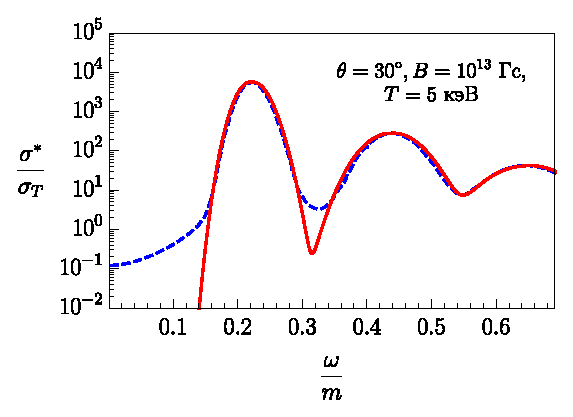
\includegraphics[width=0.32\linewidth,clip]{AliceDeltaAverageB023T001Deg30.eps}
	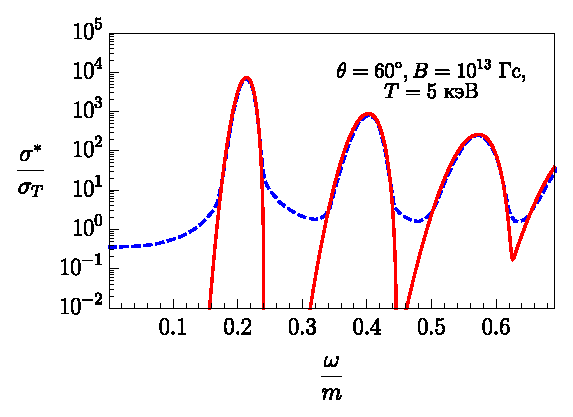
\includegraphics[width=0.32\linewidth,clip]{AliceDeltaAverageB023T001Deg60.eps}
	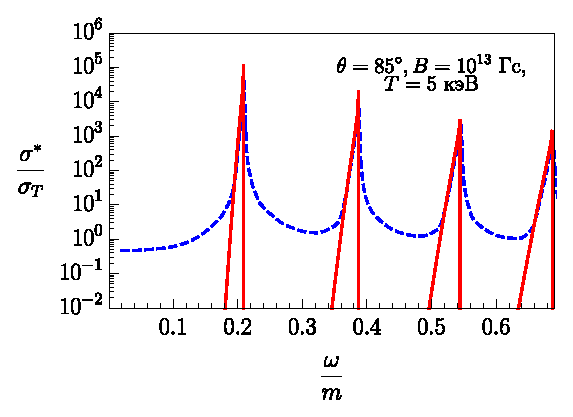
\includegraphics[width=0.32\linewidth,clip]{AliceDeltaAverageB023T001Deg85.eps}
	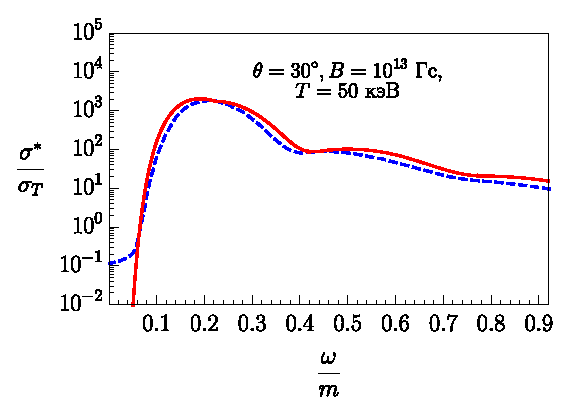
\includegraphics[width=0.32\linewidth,clip]{AliceDeltaAverageB023T01Deg30.eps}
	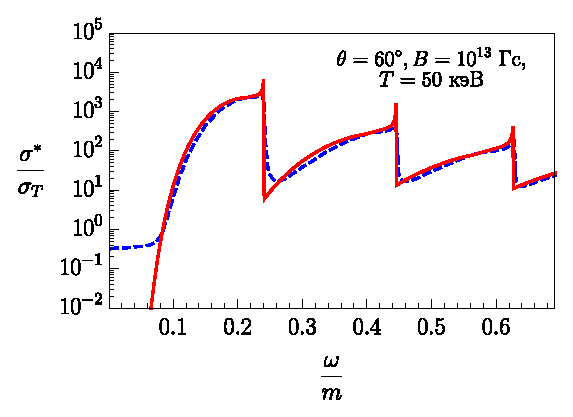
\includegraphics[width=0.32\linewidth,clip]{AliceDeltaAverageB023T01Deg60.eps}
	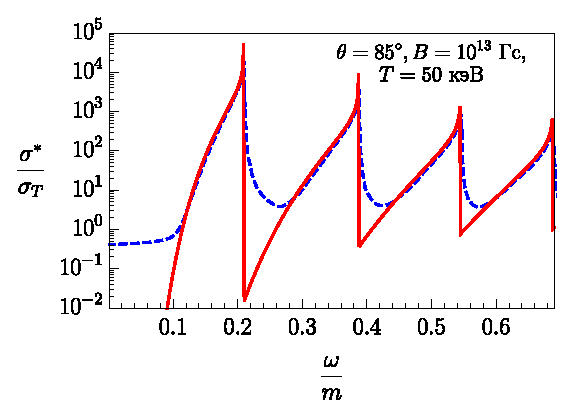
\includegraphics[width=0.32\linewidth,clip]{AliceDeltaAverageB023T01Deg85.eps}
	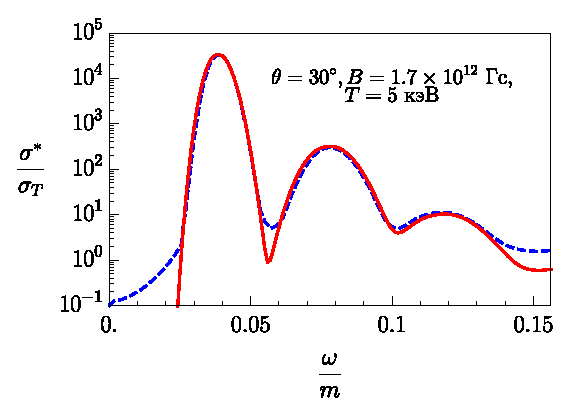
\includegraphics[width=0.32\linewidth,clip]{AliceDeltaAverageB0039T001Deg30.eps}
	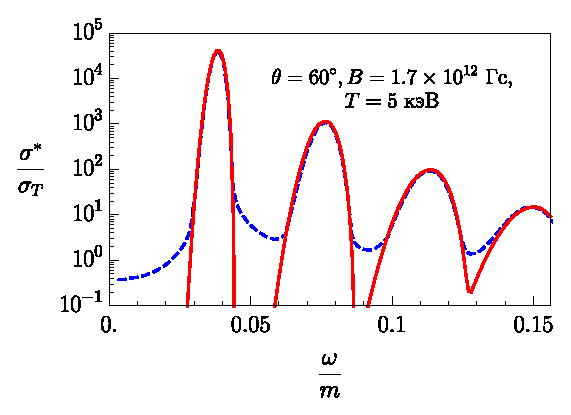
\includegraphics[width=0.32\linewidth,clip]{AliceDeltaAverageB0039T001Deg60.eps}
	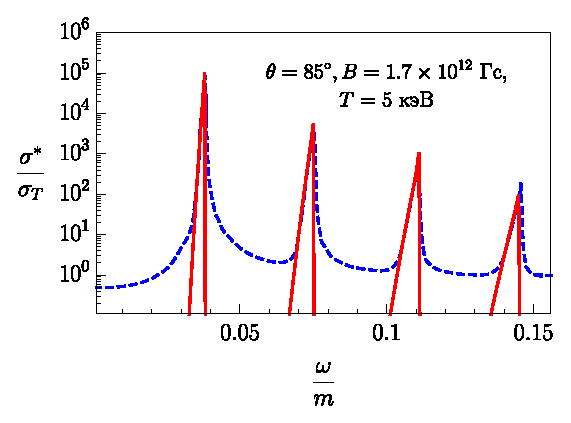
\includegraphics[width=0.32\linewidth,clip]{AliceDeltaAverageB0039T001Deg85.eps}
	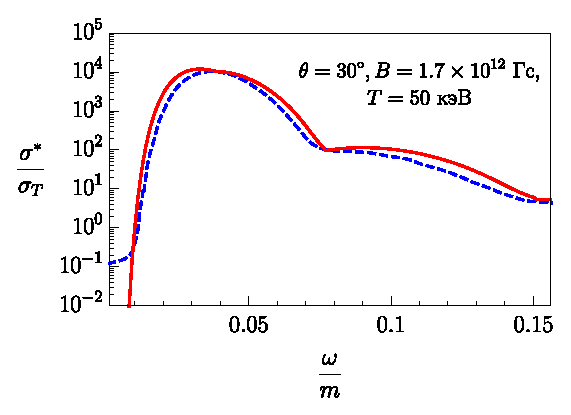
\includegraphics[width=0.32\linewidth,clip]{AliceDeltaAverageB0039T01Deg30.eps}
	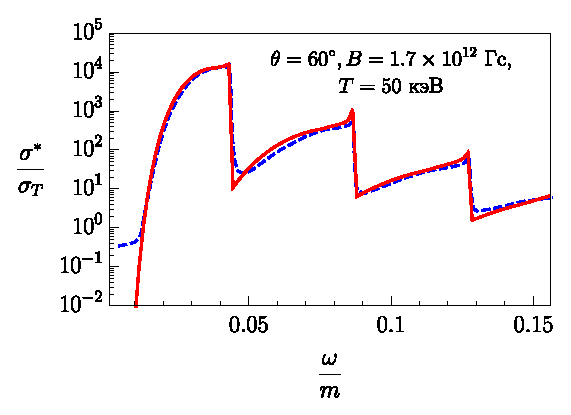
\includegraphics[width=0.32\linewidth,clip]{AliceDeltaAverageB0039T01Deg60.eps}
	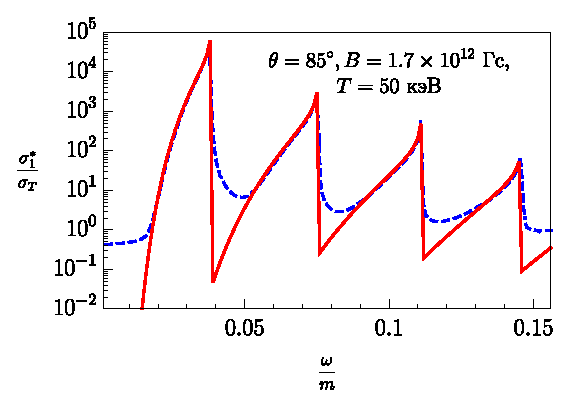
\includegraphics[width=0.32\linewidth,clip]{AliceDeltaAverageB0039T01Deg85.eps}	
	\caption{Cечения (в единицах $\sigma_T$), усредненного по поляризациям начального фотона, $e\gamma^{(2)}  \to e\gamma$, полученном в работе~\cite{Harding:1991} (пунктирная линия) и $\delta$-функциональном приближении (сплошная линия) для различных углов $\theta$ между импульсом фотона и направлением магнитного поля. Все начальные и конечные электроны находятся на основном уровне Ландау.}
	\label{fig:CompAndHardO}
\end{figure}
\clearpage
%\begin{figure}[t!]\centering
%	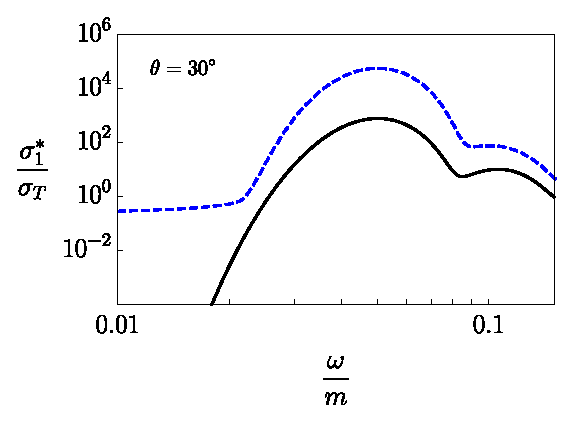
\includegraphics[width=0.5\linewidth,clip]{CompareMushOs005MushtukovX1Ground.eps}
%	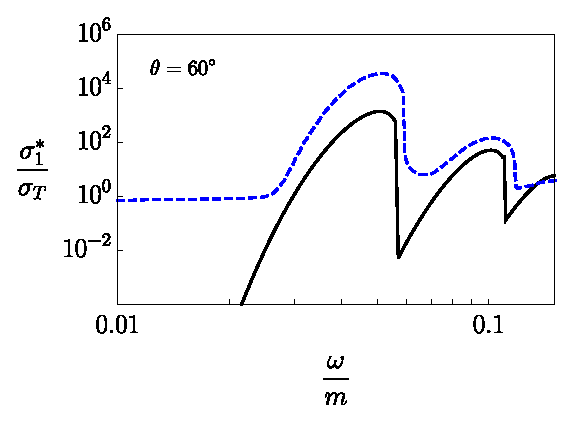
\includegraphics[width=0.5\linewidth,clip]{CompareMushOs005MushtukovX2Ground.eps}
%	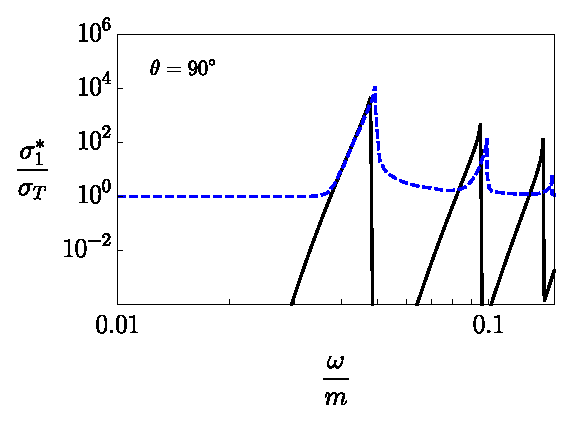
\includegraphics[width=0.5\linewidth,clip]{CompareMushOs005MushtukovX3Ground.eps}
%	\caption{Cечения (в единицах $\sigma_T$) рассеяния фотона моды 1, 
%	$e\gamma^{(1)}  \to e\gamma$, полученном в работе~\cite{Mushtukov:2016} 
%	(пунктирная линия) и $\delta$-функциональном приближении (сплошная линия) 
%	для различных углов $\theta$ между импульсом начального фотона и 
%	направлением магнитного поля (значения изображены на графиках). 
%	$B=2.2\times 10^{12}$ Гс, $T = 20$ кэВ, $\mu=0$. Начальные и конечные 
%	электроны находятся на основном уровне Ландау.}
%	\label{fig:CompAndMushXGround}
%\end{figure}
%\begin{figure}[t!]\centering
%	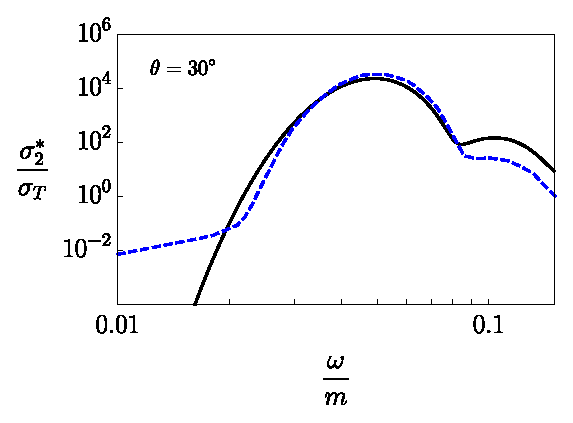
\includegraphics[width=0.5\linewidth,clip]{CompareMushOs005MushtukovO1Ground.eps}
%	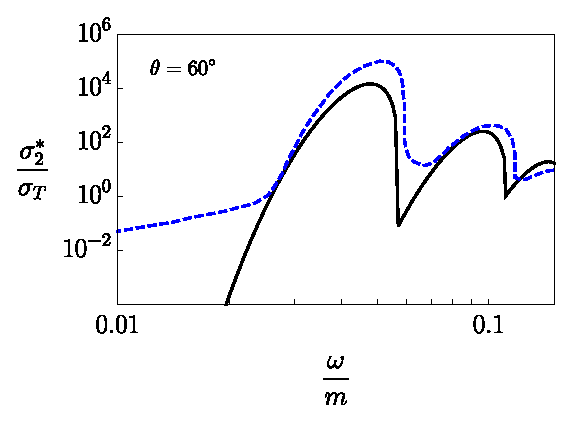
\includegraphics[width=0.5\linewidth,clip]{CompareMushOs005MushtukovO2Ground.eps}
%	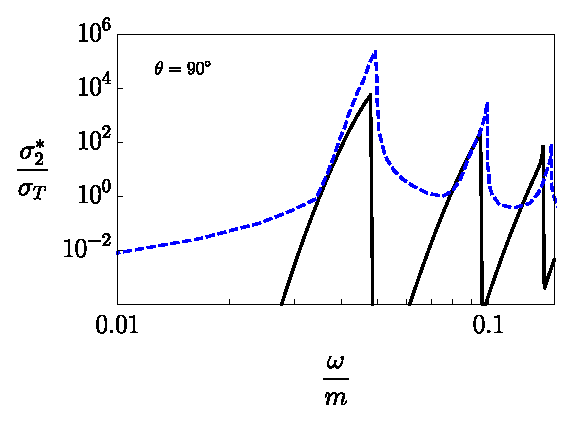
\includegraphics[width=0.5\linewidth,clip]{CompareMushOs005MushtukovO3Ground.eps}
%	\caption{То же, что и на рис.~\ref{fig:CompAndMushXGround} для параметров 
%	плазмы $B=2.2\times 10^{12}$ Гс, $T = 20$ кэВ, $\mu=0$.}
%	\label{fig:CompAndMushO}
%\end{figure}
%\clearpage
%\begin{figure}[t!]\centering
%	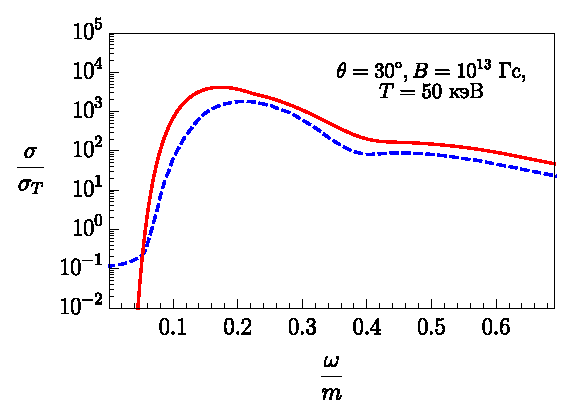
\includegraphics[width=0.55\linewidth,clip]{AliceDeltaManyLevelB023T01Deg30.eps}\\
%	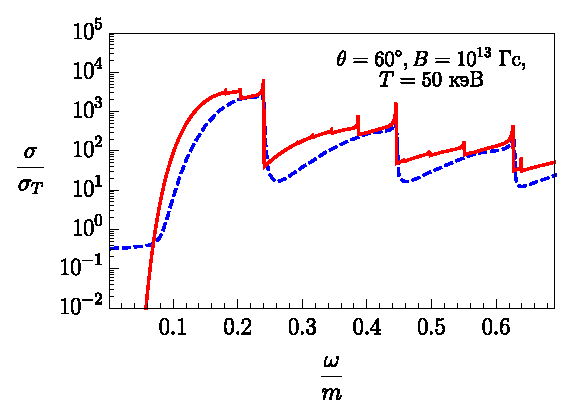
\includegraphics[width=0.55\linewidth,clip]{AliceDeltaManyLevelB023T01Deg60.eps}\\
%	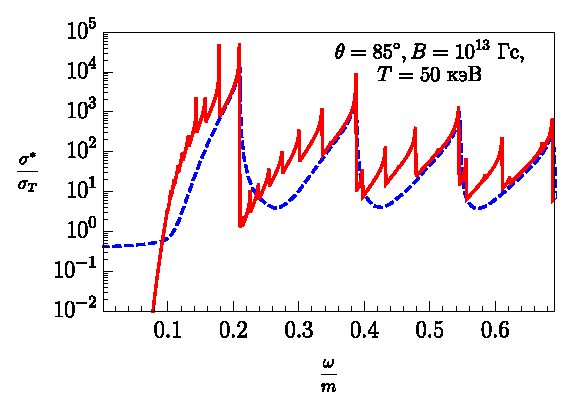
\includegraphics[width=0.55\linewidth,clip]{AliceDeltaManyLevelB023T01Deg85.eps}
%	\caption{Cечения (в единицах $\sigma_T$), усредненного по поляризациям начального фотона и по поляризациям начального электрона, $e\gamma^{(2)}  \to e\gamma$, полученном в работе~\cite{Harding:1991} (пунктирная линия) и $\delta$-функциональном приближении (сплошная линия) для различных углов $\theta$ между импульсом фотона и направлением магнитного поля. По начальным электронам взя. Значение температуры $T=50$ кэВ, а индукция магнитного поля -- $B=10^{13}$ Гс.\label{fig:HardingManyLevels}}
%\end{figure}
%\clearpage

Рассмотрим теперь ситуацию сверхсильного магнитного поля, \linebreak\mbox{$B\sim 
10^{15}-10^{16}$} Гс и высоких температур $T=1$ МэВ, которые характерны для 
гигантских вспышек SGR (источников мягких повторяющихся гамма-всплесков).  
Исследование комптоновского процесса в магнитных полях указанного масштаба было 
проведено, например, в работе~\cite{Chistyakov:2009}. Однако, полученные в этом 
исследовании результаты будут справедливыми только для области энергий фотонов 
вдали от резонансов. Поэтому представляет самостоятельный интерес вычислить 
коэффициент поглощения фотона в пределе сильного поля с учетом возможного 
резонанса на виртуальном электроне с конечной шириной резонансного пика и 
сравнить с нерезонансным пределом~\cite{Chistyakov:2009} и 
дельта-функциональным приближением~\cite{Rumyantsev:2017}. Поскольку в пределе 
сильного магнитного поля начальный и конечный электроны будут преимущественно 
занимать основной уровень Ландау, а виртуальный электрон -- первый уровень 
Ландау, то коэффициент поглощения фотона с учетом конечной ширины резонансного 
пика примет достаточно простой для вычисления вид. Поскольку в сильном 
магнитном поле энергии фотона, на которых наблюдается резонанс, 
выше, чем порог рождения $e^+e^-$ пары $q_{\mprl}^2=4m^2$ для фотона моды 2 , 
то целесообразно рассмотреть только каналы рассеяния $e\gamma^{(1)}\to 
e\gamma^{(1)}$ и $e\gamma^{(1)}\to e\gamma^{(2)}$. Следует отметить, что для 
фотона моды~1 порог рождения $e^+e^-$ пары $q_{\mprl}^2=(M_1+m)^2$ заведомо 
выше рассматриваемой области резонанса $q_{\mprl}^2=(M_1-m)^2$.

Как показывает численный анализ, в 
случае сильно замагниченной, горячей, зарядово-симметричной плазмы полная 
ширина поглощения электрона для первого уровня Ландау $\Gamma_1$ мало отличается от соответствующего 
выражения в 
сильном магнитном поле и ультрарелятивистских электронов~\cite{KM_Book_2013}:
\begin{equation}
	\begin{aligned}
		E''_1\Gamma_1=\alpha \beta
		(1-e^{-1})\simeq 0.623 \alpha \beta\, ,
	\end{aligned}
\end{equation}
где $E''_n=E+\omega$ -- энергия виртуального электрона.

 Парциальные коэффициенты поглощения фотона для каналов $e \gamma^{(1)} \to 
 e\gamma^{(1)}$ и $e \gamma^{(1)} \to e\gamma^{(2)}$ с учетом конечной ширины 
 поглощения электрона в случае, когда начальный фотон 
 распространяется поперек магнитного поля, можно 
 представить следующим образом~\textcolor{red}{в общем случае}:


\begin{equation}
	\begin{aligned}\label{Wres}
		&W_{e\gamma^{(1)}\to e\gamma^{(1)}}=\frac{\beta\alpha^2m^2}{\pi} \int 
		dQ_0dk'_z \frac{{k_z'}^2\omega } 
		{(-Q_{\mprl}^2)^2\varkappa}\exp\left[-\frac{q_\perp^2+{q'}_\perp^2}{2\beta}\right]\times
		\\
		&\times\sum_{n=1}^{\infty}\sum_{\sigma=\pm 1}\frac{1}{[(n-1)!]^2}\left(\frac{\sqrt{q_\perp^2} \sqrt{q_\perp'^2}}{2\beta}\right)^{2(n-1)}\bigg\{
		\frac{1}{((p_\sigma+q)_{\mprl}^2-M_n^2)^2+(E''_n\Gamma_n)^2}  +\\
		&+\frac{1}{((p_\sigma-q')_{\mprl}^2-M_n^2)^2+(E''_n\Gamma_n)^2}-
		\\
		&-2
		\sum_{n'=1}^{\infty}\frac{(n-1)!}{(n'-1)!}\left(\frac{\sqrt{q_\perp^2} \sqrt{q_\perp'^2}}{2\beta}\right)^{n'+n}J_{n+n'}\left(\frac{\sqrt{q_\perp^2} \sqrt{q_\perp'^2}}{\beta}\right)\times\\
		&\times\frac{[(p_\sigma+q)^2_{\mprl}-M_n^2][(p_\sigma-q')^2_{\mprl}-M^2_{n'}]+E''_n\Gamma_nE''_{n'}\Gamma_{n'}}{[((p_\sigma-q')_{\mprl}^2-M_n^2)^2+(E''_n\Gamma_n)^2][((p_\sigma+q)_{\mprl}^2-M_{n'}^2)^2+(E''_n\Gamma_{n'})^2]}
		\bigg\}\times
		\\&\times 
		f_e{(E_\sigma)}\left[1-f_e{(E_\sigma+Q_0)}\right]\left[1+f_\gamma(\omega')\right]
		 \, ,
	\end{aligned}
\end{equation}

\begin{equation}
	\begin{aligned}\label{Wres2}
		&W_{e\gamma^{(1)}\to e\gamma^{(2)}}=\frac{\beta\alpha^2m^2}{\pi} \int 
		dQ_0dk'_z \frac{q_\perp'^2\omega } 
		{(-Q_{\mprl}^2)^2\varkappa}\exp\left[-\frac{q_\perp^2+{q'}_\perp^2}{2\beta}\right]
		\times
		\\
		&\times\sum_{n=1}^{\infty}\sum_{\sigma=\pm 
		1}\frac{1}{[(n-1)!]^2}\left(\frac{\sqrt{q_\perp^2} 
		\sqrt{q_\perp'^2}}{2\beta}\right)^{2(n-1)}\frac{Q_0}{\omega}\bigg\{
		\frac{1}{((p_\sigma+q)_{\mprl}^2-M_n^2)^2+(E''_n\Gamma_n)^2}+
		\\
		&+\frac{Q_0 \omega}{ q'^2_{\mprl}}\frac{1}{((p_\sigma-q')_{\mprl}^2-M_n^2)^2+(E''_n\Gamma_n)^2}-
		\\
		&-2
		\sum_{n'=1}^{\infty}\frac{(n-1)!}{(n'-1)!}\left(\frac{\sqrt{q_\perp^2} \sqrt{q_\perp'^2}}{2\beta}\right)^{n'+n} J_{n+n'}\left(\frac{\sqrt{q_\perp^2} \sqrt{q_\perp'^2}}{\beta}\right)\times\\
		&\times\frac{[(p_\sigma+q)^2_{\mprl}-M_n^2][(p_\sigma-q')^2_{\mprl}-M^2_{n'}]+E''_n\Gamma_nE''_{n'}\Gamma_{n'}}{[((p_\sigma-q')_{\mprl}^2-M_n^2)^2+(E''_n\Gamma_n)^2][((p_\sigma+q)_{\mprl}^2-M_{n'}^2)^2+(E''_n\Gamma_{n'})^2]}
		\times\\&\times
		\frac{Q_0(\omega-Q_0)}{q'^2_\perp}
		\bigg\}f_e{(E_\sigma)}\left[1-f_e{(E_\sigma+Q_0)}\right]\left[1+f_\gamma(\omega')\right]
		 \, ,
	\end{aligned}
\end{equation}

\begin{equation}
	\begin{aligned}\label{Wresalt}
		&W_{e\gamma^{(1)}\to e\gamma^{(1)}}=\frac{\beta\alpha^2m^2}{\pi} \int 
		dQ_0dk'_z \frac{{k_z'}^2\omega } 
		{(-Q_{\mprl}^2)^2\varkappa}\exp\left[-\frac{q_\perp^2+{q'}_\perp^2}{2\beta}\right]\times
		\\
		&\times\sum_{\sigma=\pm 1}\bigg\{
		\frac{1}{((p_\sigma+q)_{\mprl}^2-M_1^2)^2+(E''_1\Gamma_1)^2}  +\frac{1}{((p_\sigma-q')_{\mprl}^2-M_1^2)^2+(E''_1\Gamma_1)^2}-
		\\
		&-2
		\frac{q_\perp^2 q_\perp'^2}{4\beta^2}J_{2}\left(\frac{\sqrt{q_\perp^2} \sqrt{q_\perp'^2}}{\beta}\right)\times\\
		&\times\frac{[(p_\sigma+q)^2_{\mprl}-M_1^2][(p_\sigma-q')^2_{\mprl}-M^2_{1}]+(E''_1\Gamma_{1})^2}{[((p_\sigma-q')_{\mprl}^2-M_1^2)^2+(E''_1\Gamma_1)^2][((p_\sigma+q)_{\mprl}^2-M_{1}^2)^2+(E''_1\Gamma_{1})^2]}
		\bigg\}\times
		\\&\times 
		f_e{(E_\sigma)}\left[1-f_e{(E_\sigma+Q_0)}\right]\left[1+f_\gamma(\omega')\right]
		\, ,
	\end{aligned}
\end{equation}

\begin{equation}
	\begin{aligned}\label{Wres2alt}
		&W_{e\gamma^{(1)}\to e\gamma^{(2)}}=\frac{\beta\alpha^2m^2}{\pi} \int 
		dQ_0dk'_z \frac{q_\perp'^2\omega } 
		{(-Q_{\mprl}^2)^2\varkappa}\exp\left[-\frac{q_\perp^2+{q'}_\perp^2}{2\beta}\right]
		\times
		\\
		&\times\sum_{\sigma=\pm 
			1}\frac{Q_0}{\omega}\bigg\{
		\frac{1}{((p_\sigma+q)_{\mprl}^2-M_1^2)^2+(E''_1\Gamma_1)^2}+\frac{Q_0 \omega}{ q'^2_{\mprl}}\frac{1}{((p_\sigma-q')_{\mprl}^2-M_1^2)^2+(E''_1\Gamma_1)^2}-
		\\
		&-2
		\frac{q_\perp^2 q_\perp'^2}{4\beta^2} J_{2}\left(\frac{\sqrt{q_\perp^2} \sqrt{q_\perp'^2}}{\beta}\right)\times\\
		&\times\frac{[(p_\sigma+q)^2_{\mprl}-M_1^2][(p_\sigma-q')^2_{\mprl}-M^2_{1}]+(E''_1\Gamma_1)^2}{[((p_\sigma-q')_{\mprl}^2-M_1^2)^2+(E''_1\Gamma_1)^2][((p_\sigma+q)_{\mprl}^2-M_{1'}^2)^2+(E''_1\Gamma_{1'})^2]}
		\times\\&\times
		\frac{Q_0(\omega-Q_0)}{q'^2_\perp}
		\bigg\}f_e{(E_\sigma)}\left[1-f_e{(E_\sigma+Q_0)}\right]\left[1+f_\gamma(\omega')\right]
		\, ,
	\end{aligned}
\end{equation}
\noindent где $J_n(x)$ -- функция Бесселя целого индекса, 
\mbox{$\varkappa = \sqrt{1 - 4m^2/Q^2_{\mprl}}$, 
	$E_\sigma=\sqrt{p_{z\sigma}^2+m^2}$}, $p_{z\sigma}$ -- корни уравнения 
$Q_0+E_\sigma-E'_\sigma=0$:
\begin{equation}\label{savelaw}
	p_{z\sigma}=-\frac{Q_z}{2}+ \sigma Q_0 \varkappa\, ,
\end{equation}
$p^\alpha_{\sigma\mprl}=(E_\sigma,p_{z\sigma})$. 
Поперечная составляющая импульса конечного фотона определяется из уравнения 
дисперсии:
\begin{equation}
	q'^2_{\mprl}=q'^{2}_\perp + {\cal P}^{(\lambda)}(q') .
\end{equation}

Имеет смысл провести сравнительный анализ результатов работы \cite{Chistyakov:2009}  с резонансным случаем (\ref{Wres}) и (\ref{Wres2}) для зарядово-симметричной плазмы и поперечного направления распространения импульса фотона по отношению к внешнему магнитному полю для различных значений величины магнитного поля, температуры и энергии начального фотона.

На рис.~\ref{Graph11B200T1}--\ref{Graph11B20T1} показан  коэффициент поглощения $W_{1\to1}$ рассеяния при температуре $T=1 $~МэВ и величине магнитного поля $B=200B_e$ и $B=20B_e$ соответственно. Как видно из рис.~\ref{Graph11B200T1}--\ref{Graph11B20T1}, коэффициент поглощения для канала $\gamma^{(1)}e\to\gamma^{(1)}e$ согласуется с соответствующими результатами для предела сильного поля и отсутствия резонанса, полученными в работе \cite{Chistyakov:2009} вплоть до энергий начального фотона  $\omega\simeq3$~МэВ для поля $B=200B_e$ и  $\omega\simeq0.3$~МэВ для поля $B=20B_e$. Отсюда вытекает ограничение на применимость результатов работы \cite{Chistyakov:2009} по энергиям начального фотона. Аналогичная ситуация наблюдается и для канала $\gamma^{(1)}e\to\gamma^{(2)}e$ (см. рис. \ref{Graph12B200T1}--\ref{Graph12B20T1}).  На рис. \ref{Graph11B20T1} и \ref{Graph12B20T1} наиболее ярко видно завышение коэффициента поглощения даже при относительно малых энергиях начального фотона. Этот факт связан с тем, что в пределе сильного магнитного поля разложение амплитуды комптоновского процесса по обратным степеням поля уже не будет правомочным.  

Следует отметить   что при относительно малых температурах $T\lesssim50$ кэВ с 
тем же магнитным полем $\delta$-аппроксимация работает хуже из-за уменьшения 
области резонанса. В целом $\delta$-функциональное приближение достаточно 
хорошо будет описывать лишь первый резонансный пик.

\begin{figure}[t!]\centering
	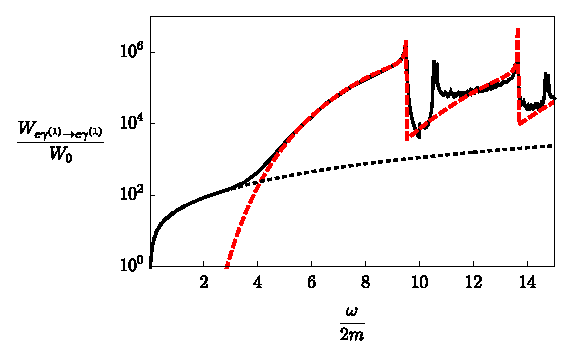
\includegraphics[width=0.8\linewidth]{Splot112001.eps}
	\caption{Зависимость коэффициента поглощения от энергии начального фотона для канала $e\gamma^{(1)}\to e\gamma^{(1)}$ при поле $B=200 B_e$ и температуре T=1 МэВ: сплошная линия -- коэффициент поглощения с учетом резонанса; штриховая линия -- без учета резонанса; пунктирная линия -- дельта-функциональное приближение. Здесь $W_0=(\alpha/\pi)^3m\simeq 3.25\cdot10^2$ см$^{-1}$.}
	\label{Graph11B200T1}
\end{figure}

\begin{figure}[t!]\centering
	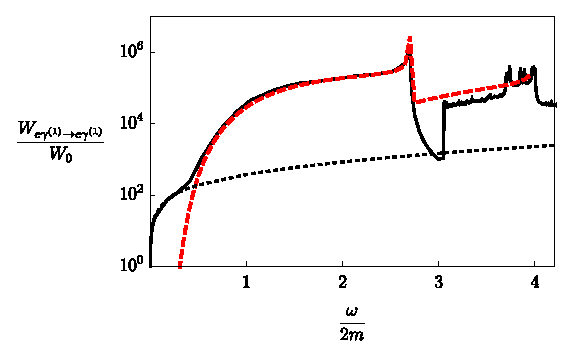
\includegraphics[width=0.8\linewidth]{Splot11201.eps}
	\caption{Зависимость коэффициента поглощения от энергии начального фотона для канала $e\gamma^{(1)}\to e\gamma^{(1)}$ при поле $B=20 B_e$ и температуре T=1 МэВ. Обозначение для линий то же, что и для рис. \ref{Graph11B200T1}.}
	\label{Graph11B20T1}
\end{figure}

\begin{figure}[t!]\centering
	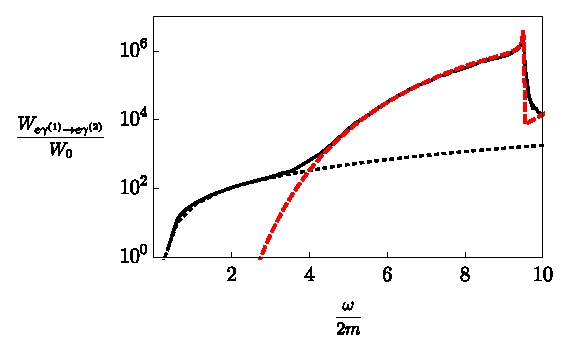
\includegraphics[width=0.8\linewidth]{Splot122001.eps}
	\caption{Зависимость коэффициента поглощения от энергии начального фотона для канала $e\gamma^{(1)}\to e\gamma^{(2)}$ при поле $B=200 B_e$ и температуре T=1 МэВ. Обозначение для линий то же, что и для рис. \ref{Graph11B200T1}.}
	\label{Graph12B200T1}
\end{figure}

\begin{figure}[t!]\centering
	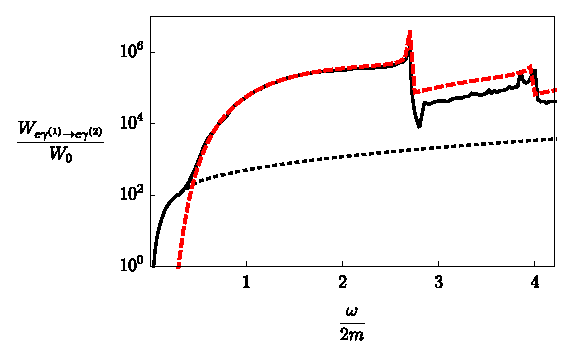
\includegraphics[width=0.8\linewidth]{Splot12201.eps}
	\caption{Зависимость коэффициента поглощения от энергии начального фотона для канала $e\gamma^{(1)}\to e\gamma^{(2)}$ при поле $B=20 B_e$ и температуре T=1 МэВ. Обозначение для линий то же, что и для рис. \ref{Graph11B200T1}.}
	\label{Graph12B20T1}
\end{figure}
\clearpage
